\documentclass[border=6pt]{standalone}
% Shared preamble for web figures.  Each figure is a standalone .tex that
% \input's this file; scripts/make-figures.sh turns it into an SVG.
% Handouts pull the same file with \fig{Unit_X/<name>}.
\usepackage[T1]{fontenc}
\usepackage{helvet}
\renewcommand{\familydefault}{\sfdefault}
\renewcommand{\ttdefault}{pcr}  % Courier: a real Type 1 typewriter font
\usepackage{amsmath}
\usepackage{tikz}
\usetikzlibrary{arrows.meta,positioning,calc,shapes.symbols,shapes.geometric}

% Who makes the rules is the point of most diagrams in this book, so the
% colors mean the same thing everywhere: blue is a person, orange is the
% computer, green is an answer, pink is the human brain.
\definecolor{person}{HTML}{2C6FAE}
\definecolor{machine}{HTML}{D35400}
\definecolor{result}{HTML}{1E8449}
\definecolor{brainpink}{HTML}{C2185B}
\definecolor{ink}{HTML}{2C3E50}

\tikzset{
  doodle/.style={line width=1.5pt, line cap=round, line join=round, draw=ink},
  box/.style={draw, rounded corners=5pt, line width=1.1pt, align=center,
              inner sep=7pt, minimum height=1.0cm, font=\small},
  personbox/.style={box, draw=person, fill=person!10},
  machinebox/.style={box, draw=machine, fill=machine!10},
  resultbox/.style={box, draw=result, fill=result!10},
  plainbox/.style={box, draw=ink!70, fill=ink!4},
  flow/.style={-{Stealth[length=8pt]}, line width=1.4pt, draw=ink},
}

% A person (blue) and a robot head (orange) as small icons.
% \personicon{x}{y}{scale}   \roboticon{x}{y}{scale}
\newcommand{\personicon}[3]{%
  \begin{scope}[shift={(#1,#2)}, scale=#3]
    \fill[person] (0,0.62) circle (0.28);
    \fill[person, rounded corners=6pt] (-0.42,-0.55) rectangle (0.42,0.28);
  \end{scope}}
\newcommand{\roboticon}[3]{%
  \begin{scope}[shift={(#1,#2)}, scale=#3]
    \draw[machine, line width=1.2pt] (0,0.5) -- (0,0.72);
    \fill[machine] (0,0.78) circle (0.08);
    \draw[machine, line width=1.4pt, fill=machine!12, rounded corners=4pt] (-0.5,-0.45) rectangle (0.5,0.5);
    \fill[ink] (-0.2,0.12) circle (0.08);
    \fill[ink] (0.2,0.12) circle (0.08);
    \draw[ink, line width=1pt] (-0.22,-0.22) -- (0.22,-0.22);
  \end{scope}}

\begin{document}
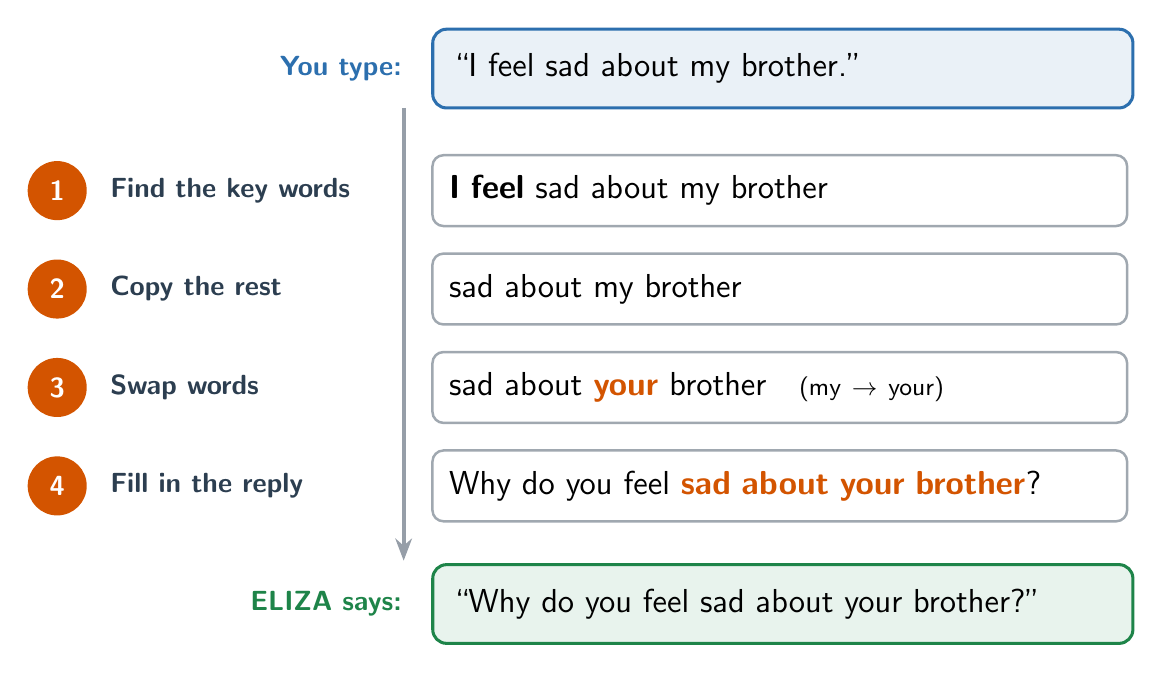
\begin{tikzpicture}[
  stepdot/.style={circle, fill=machine, text=white, font=\bfseries, minimum size=0.75cm, inner sep=0pt},
  what/.style={anchor=west, font=\bfseries, text=ink, text width=3.6cm},
  card/.style={anchor=west, draw=ink!45, fill=white, rounded corners=4pt, line width=0.9pt,
               inner sep=6pt, minimum height=0.9cm, font=\large, text width=8.4cm},
]
% How ELIZA answers one sentence, using only rules a person wrote.
\node[personbox, anchor=west, font=\large, text width=8.4cm, align=left] (in) at (4.75,1.5) {``I feel sad about my brother.''};
\node[anchor=east, font=\bfseries, text=person] at (4.5,1.5) {You type:};

\foreach \n/\w/\t/\y in {
  1/{Find the key words}/{\textbf{I feel} sad about my brother},
  2/{Copy the rest}/{sad about my brother},
  3/{Swap words}/{sad about \textcolor{machine}{\textbf{your}} brother \ \ {\small(my \(\to\) your)}},
  4/{Fill in the reply}/{Why do you feel \textcolor{machine}{\textbf{sad about your brother}}?}} {
  \pgfmathsetmacro{\yy}{-0.05-1.25*(\n-1)}
  \node[stepdot] at (0,\yy) {\n};
  \node[what] at (0.55,\yy) {\w};
  \node[card] at (4.75,\yy) {\t};
}
\node[resultbox, anchor=west, font=\large, text width=8.4cm, align=left] (out) at (4.75,-5.3) {``Why do you feel sad about your brother?''};
\node[anchor=east, font=\bfseries, text=result] at (4.5,-5.3) {ELIZA says:};
\draw[flow, draw=ink!50] (4.4,1.0) -- (4.4,-4.75);
\end{tikzpicture}
\end{document}
